%\begin{frame}
%  \frametitle{Originators of \texttt{libMesh}}
%  \begin{block}{}
%    \begin{itemize}
%    \item 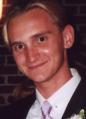
\includegraphics[scale=3]{benkirk} Benjamin S. Kirk, NASA Johnson Space Center
%    \item 
\includegraphics[scale=0.35]{jwpeterson} John W. Peterson, Idaho National Lab
%    \item 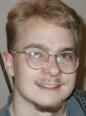
\includegraphics[scale=0.35]{roystgnr} Roy H. Stogner, University of Texas at Austin
%    \end{itemize}
%  \end{block}
%
%\end{frame}

\frame
{
  \frametitle{Thanks to Dr.\ Graham F.\ Carey}

  \begin{columns}
    \begin{column}{.55\textwidth}
      \scriptsize
      \begin{quote}
        The original development team was heavily influenced by Professor Graham F. Carey, professor of aerospace engineering and engineering mechanics at The University of Texas at Austin, director of the ICES Computational Fluid Dynamics Laboratory, and holder of the Richard B. Curran Chair in Engineering.

        Many of the technologies employed in libMesh were implemented because Dr. Carey taught them to us, we went back to the lab, and immediately began coding. In a very real way, he was ultimately responsible for this library that we hope you may find useful, despite his continued insistence that ``no one ever got a PhD from here for writing a code.''
      \end{quote}
\normalsize
    \end{column}
    \begin{column}{.45\textwidth}
      \includegraphics[width=\textwidth]{grahamcarey}
    \end{column}
  \end{columns}
}


\begin{frame}
\frametitle{Acknowledgements}

Recent libMesh contributors:
\begin{columns}

\column{.45\textwidth}

\begin{itemize}
\item David Andrs
\item Paul Bauman
\item Vikram Garg
\item Derek Gaston
\item Dmitry Karpeev
\end{itemize}

\column{.45\textwidth}
\begin{itemize}
\item Benjamin Kirk
\item David Knezevic
\item Cody Permann
\item John Peterson
\item Sylvain Vallaghe
\end{itemize}

\end{columns}

\vspace{5mm}

Useful resources:
\begin{itemize}
\item libMesh: \url{https://libmesh.github.io/}
\item MOOSE: \url{https://mooseframework.org/}
\item FALCON: \url{https://github.com/idaholab/falcon}
\item MASA: \url{https://manufactured-solutions.github.io/MASA/}
\item GRINS: \url{https://grinsfem.github.io/}
\item Akselos: \url{http://www.akselos.com/}
\end{itemize}


\end{frame}


